\section{Journal Extension: Coverage, Failure, and Cost Diagnostics}\label{sec:diagnostics}
\subsection{Candidate coverage separates retrieval from selection}
Saved feature and ranking records let us reconstruct candidate membership and evaluate~\eqref{eq:coverage_ceiling} for dense sixty-four, hybrid fifteen, and the expanded union where available. We check pool sizes, subset inclusion, and parent IDs independently of historical field names before computing coverage. No new rankings are created.

\begin{table*}[t]
\centering\small
\caption{New secondary analysis of saved candidate pools. Judged coverage includes every positively judged parent in the pool. The Recall@8 ceiling additionally enforces the eight-output budget and relaxes relevance-score and prefix constraints. Values are query means.}
\label{tab:coverage}\begin{tabular}{llrrr}
\toprule
Dataset & Pool & Mean size & Judged coverage & Recall@8 ceiling\\
\midrule
SciFact & Dense 64 & 64.00 & 0.9243 & 0.9243\\
SciFact & Hybrid 15 & 15.00 & 0.8569 & 0.8569\\
SciFact & Expanded union & 22.30 & 0.8903 & 0.8903\\
NFCorpus & Dense 64 & 64.00 & 0.2666 & 0.2375\\
NFCorpus & Hybrid 15 & 15.00 & 0.1780 & 0.1725\\
NFCorpus & Expanded union & 20.29 & 0.2028 & 0.1942\\
FiQA & Dense 64 & 64.00 & 0.6489 & 0.6483\\
FiQA & Hybrid 15 & 15.00 & 0.4824 & 0.4824\\
\bottomrule
\end{tabular}

\end{table*}

Table~\ref{tab:coverage} and Fig.~\ref{fig:coverage} show how much candidate opportunity differs by collection. SciFact's ceiling is \scifactShortCeiling{} for hybrid fifteen and \scifactUnionCeiling{} for the expanded union. The corresponding NFCorpus ceilings are \nfcorpusShortCeiling{} and \nfcorpusUnionCeiling{}. FiQA's base shortlist has a ceiling of \fiqaShortCeiling{}, compared with \fiqaDenseCeiling{} for dense sixty-four. These are optimistic opportunities under the judgments, not predictions of a learned reranker's performance.

For \scifactNoRelevant{} SciFact, \nfcorpusNoRelevant{} NFCorpus, and \fiqaNoRelevant{} FiQA queries, the hybrid shortlist contains no positively judged parent. An eight-of-fifteen selector cannot improve judged recall on those queries without different candidates. Expansion recovers some exclusions in the protected datasets, but stays inside dense sixty-four and cannot recover a corpus document missing from that set.

\begin{figure*}[t]
\centering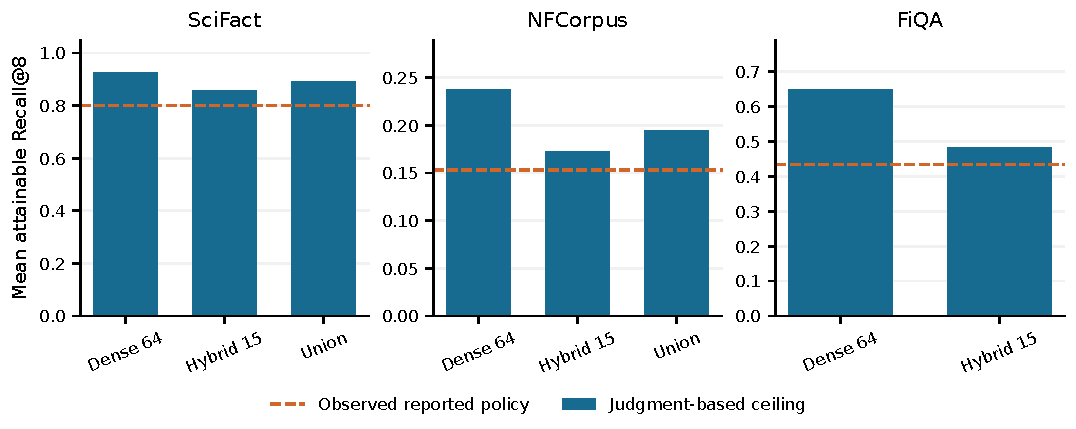
\includegraphics[width=\textwidth]{candidate_coverage.pdf}
\caption{New judgment-based Recall@8 ceilings for the saved candidate pools, compared with the observed reported-policy recall. The dashed line is the same policy within each dataset panel. Expanded-union ceilings relax the protected-prefix and tail-score constraints and therefore do not measure pure search inefficiency.}
\label{fig:coverage}
\end{figure*}

The number of judged-relevant documents also changes the scale of Recall@8. Even eight perfect outputs recover only a fraction of a large relevant set. NFCorpus contains queries with substantially larger relevant sets than the single-evidence cases common in SciFact; its lower recall reflects task structure as well as candidate opportunity and ranking performance. Comparing policies on the same queries, against the relevant candidate ceiling, helps separate these factors.

The union widens the relaxed opportunity set, but the actual task commits five positions to the original head and requires replacements to satisfy neural-score dominance. Redundancy remains a proxy for complementary evidence. The gap to the union ceiling therefore reflects constraints and model errors as well as the finite search budget.

\subsection{Mean improvements coexist with individual losses}
Table~\ref{tab:query_outcomes} counts changes from the reference policy after seed averaging within each query. Against base GAS, SciFact has \scifactWins{} recall gains, \scifactLosses{} losses, and \scifactTies{} ties; NFCorpus has \nfcorpusWins{} gains, \nfcorpusLosses{} losses, and \nfcorpusTies{} ties. The favorable NFCorpus mean thus includes queries that lose recall. FiQA has no recall changes beyond the tie tolerance against L6-only, although some memberships and redundancy values differ.

\begin{table*}[t]
\centering\small\setlength{\tabcolsep}{4pt}
\caption{New query-level outcome and seed-stability analysis. References are base GAS for SciFact/NFCorpus and L6-only for FiQA. Counts use a $10^{-12}$ numerical tie tolerance. Seed-varying ranks count queries with more than one final ordered list among the five saved seeds.}
\label{tab:query_outcomes}\begin{tabular}{lrrrrrr}
\toprule
Dataset & Recall wins & Ties & Losses & Lower redundancy & Seed-varying ranks & Seed-varying recall\\
\midrule
SciFact & 2 & 293 & 5 & 158 & 0 & 0\\
NFCorpus & 15 & 295 & 13 & 135 & 29 & 3\\
FiQA & 0 & 648 & 0 & 6 & 7 & 0\\
\bottomrule
\end{tabular}

\end{table*}

Redundancy falls for \scifactLowerRed{} SciFact queries and \nfcorpusLowerRed{} NFCorpus queries, and rises for none, consistent with Proposition~\ref{prop:safety}. The paired changes in Fig.~\ref{fig:paired} show many zeros and a small subset with recall differences. A mean does not show how those outcomes are distributed.

\begin{figure*}[t]
\centering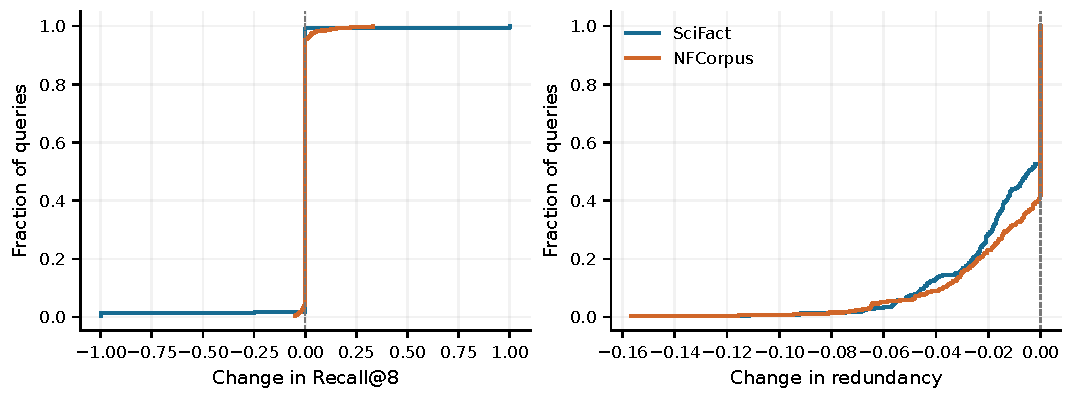
\includegraphics[width=\textwidth]{paired_distributions.pdf}
\caption{New empirical cumulative distributions of query-level refinement-minus-base differences. Recall changes can be positive or negative. Nonpositive redundancy changes follow the refinement acceptance rule. Seeds are averaged within queries before these distributions are constructed.}
\label{fig:paired}
\end{figure*}

The following extreme cases were chosen deterministically to illustrate the risk, not to represent the full test set. SciFact query 384 has one positively judged relevant parent. Base recall is 1 and refined recall is 0, although the candidate-pool ceiling is 1 and the top five are unchanged. The only relevant output was lost below the protected head. Redundancy fell by approximately 0.04373 even as judged retrieval worsened.

For NFCorpus query PLAIN-2570, the judgments contain 40 relevant parents. Base Recall@8 is 0.075 and refined Recall@8 is 0.025, or three versus one positively judged output. Mean redundancy falls by approximately 0.09454, while the relaxed Recall@8 ceiling is 0.125 for both the original and expanded pools. Candidate opportunity alone does not explain the loss; admissibility, relevance estimates, and the objective also matter. The fixed retrospective selection rule used lowest paired recall change, then largest redundancy decrease, then query ID.

Protecting a top-five metric can serve an application that values that prefix, but it does not establish that the remaining evidence can be replaced safely. A mean-retention threshold may hide a severe loss on an individual query. Recall distributions, the number of harmed queries, and their application-specific costs should accompany the mean.

\subsection{Seed stability is a property of outputs, not independent evidence}
Across seeds, final rankings differ on \scifactSeedVary{} SciFact, \nfcorpusSeedVary{} NFCorpus, and \fiqaSeedVary{} FiQA queries. Recall varies on \scifactSeedRecall{}, \nfcorpusSeedRecall{}, and \fiqaSeedRecall{} queries, respectively. Different sampled trajectories can lead to the same final output; the five-seed average does not by itself describe that distinction.

Stable outputs do not create independent queries, and different tail documents can share a judged status without changing recall. On NFCorpus, more queries have varying ordered lists than varying recall. The complete seed export retains scores and search statuses, allowing this difference to be inspected directly rather than inferred from aggregate variance.

When stochastic search repeatedly reaches an output also found by matched greedy and exact methods, the result does not identify randomness or amplitude amplification as the unique cause of the effectiveness gain. It does describe this implementation's stability under the recorded budgets and seeds.

\subsection{Additive cost attribution and the scope for selector acceleration}
For each primary seeded request, the journal exporter reconstructs
\begin{align}
T_{\mathrm{online}}={}&T_{\mathrm{upstream}}+T_{\mathrm{L6,original}}
+T_{\mathrm{L6,extra}}\nonumber\\
&+T_{\mathrm{base}}+T_{\mathrm{refine}}.
\label{eq:cost_composition}
\end{align}
Upstream time covers query encoding, dense search, representative features, and applicable lexical/hybrid/union processing. Extra inference and refinement are zero for the FiQA base. We check each sum against the saved request total before taking means. Composed stage measurements are additive; separately measured percentiles are not necessarily so.

\begin{figure*}[t]
\centering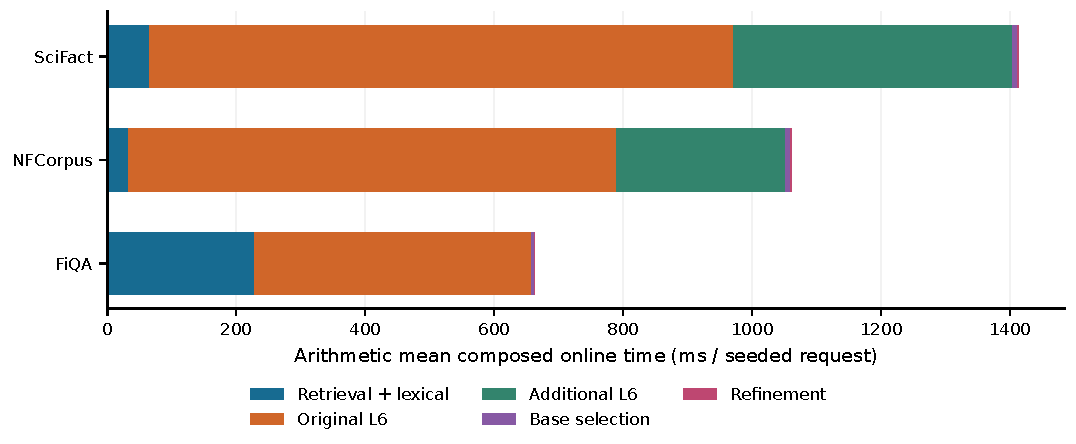
\includegraphics[width=\textwidth]{cost_decomposition.pdf}
\caption{New decomposition of arithmetic mean online time using additive per-request components. Small selector segments are retained. The plot uses means for additivity; Table~\ref{tab:latency} separately reports request-level medians and P95 values. Differences between collection sessions are not controlled cross-session speed experiments.}
\label{fig:cost}
\end{figure*}

In Fig.~\ref{fig:cost}, original L6 inference accounts for \scifactOriginalLsixShare\%, \nfcorpusOriginalLsixShare\%, and \fiqaOriginalLsixShare\% of the respective primary mean online times. Additional L6 scoring further dominates the refined pipelines. Base-plus-refinement selection accounts for \scifactSelectorShare\%, \nfcorpusSelectorShare\%, and \fiqaSelectorShare\%, respectively. Even an idealized removal of all measured selector time would leave most of the composed request cost.

For $f=\overline{T}_{\mathrm{selector}}/\overline{T}_{\mathrm{online}}$, a hypothetical zero-time selector with unchanged upstream stages could reduce the mean by fraction $f$. The idealized speedup would be $1/(1-f)$. This bound accounts for the same staged computation; it is not a hardware prediction. A practical quantum implementation would still need state preparation, data access, reversible arithmetic, and measurement. Within the measured cost boundary, reduced selection phase counts alone give little support to an end-to-end acceleration claim.
